\begin{frame}{Differences to 1G (NMT)}
  \begin{itemize}
    \item Much larger committee
    \item Many people working on NMT worked on GSM also 
    \item More interference by countries and companies
    \item Technical development similar
  \end{itemize}
\end{frame}

\begin{frame}{GSM History}
 \begin{chrono}[10]{1982}{1992}{3ex}{\textwidth}
   \event{1982}{CEPT started GSM Committee}
   \event[1982]{1987}{Different technologies and proposals presented}
   \event{1987}{\emph{memorandum of understanding} (13 states)}
   \event{1988}{CEPT was replaced by ETSI}
   \event[1990]{1993}{Siemens, Alcatel, Nokia and Ericsson enter cross-license agreement with Motorola}
   \event{1992}{Introduction of system in Europe}
 \end{chrono}
\end{frame} 
  

%  \begin{description}
%    \item[1982] CEPT started GSM %CEPT was only open for operators
%    \item[1982-1987] Different technologies and proposals presented.
%    \item[1987] \emph{memorandum of understanding} (13 states)
%    \begin{itemize}
%      \item No \emph{general architecture patenting} or \emph{non-disclosure patenting strategy}
%    \end{itemize}
%    \item[1988] CEPT was replaced by ETSI %Also open for manufacturers and privately owned operators
%    \begin{itemize}
%      \item Members have to notify essential IPRs
%      \begin{itemize}
%        \item 140 distinct IPRs in 1998
%      \end{itemize} 
%      \item Motorola: \emph{license without general declaration}
%      \item Others: \emph{gentleman's agreement}
%    \end{itemize}
%    \item[1990-1993] Siemens, Alcatel, Nokia and Ericsson enter cross-license agreement with Motorola
%    \item[1993] \emph{licensing-by-default} (abandoned due to complaints)
%    \item[Next Policy] Members report IPRs, ETSI negotiates conditions
%    \item[1994] GSM became big success
%  \end{description}

\begin{frame}{Standardisation Phases}
  \begin{itemize}
    \item \textbf{Pre-standardisation Phase:}
    \begin{itemize}
      \item Until Feb. 1987
      \item different technologies and proposals
      \item first without clear vision, later with standard goal in mind
      \item No ownership intensification
    \end{itemize}
    \item \textbf{Standard Production Phase:}
    \begin{itemize}
      \item Feb. 1987 - 1991
      \item Exact implementation decided
      \item product development
      \item Motorola intensified patenting, others refrained
    \end{itemize}
    \item \textbf{Standard Diffusion Phase:}
    \begin{itemize}
      \item After 1991
      \item new services and additions
    \end{itemize}
  \end{itemize}
\end{frame}

\begin{frame}{Essential IPRs}
  \begin{columns}
      \begin{column}{0.55\textwidth}
          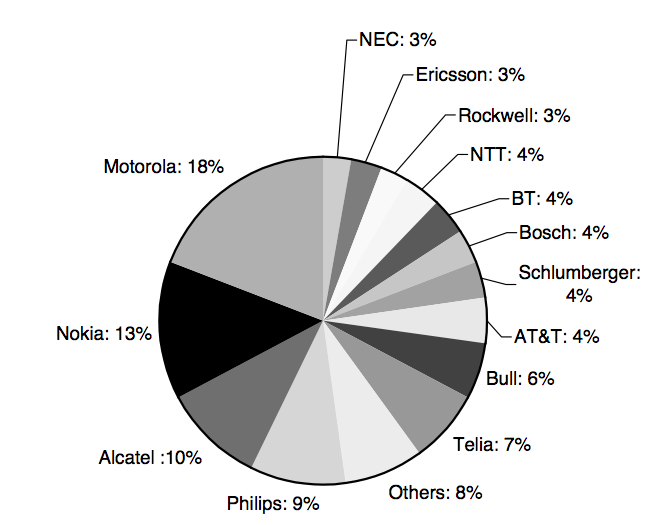
\includegraphics[width=\textwidth]{pictures/iprs}
      \end{column}
      \hfill
    
      \begin{column}{0.45\textwidth}
          \begin{itemize}
              \item 140 essential IPRs
              \item Motorola refuses general licensing
              \item Licence fees needed for continuous revenue
              \item Cross-licensing with Siemens, Alcatel, Nokia and Ericsson
          \end{itemize}
      \end{column}
      \end{columns}
\end{frame}

\begin{frame}{Market Shares}
  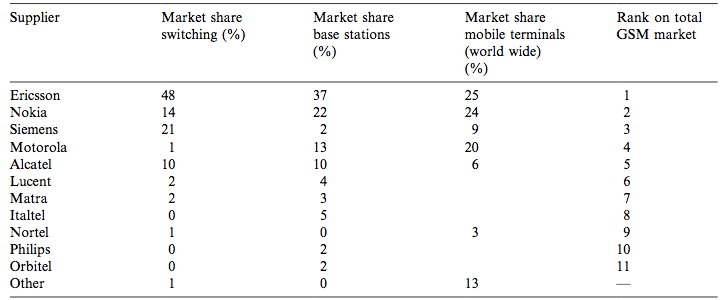
\includegraphics[width=\textwidth]{pictures/2gmarketshares}
  
  Motorola, Siemens, Alcatel, Nokia and Ericsson held $85\%$ of the market shares in 1996.
\end{frame}


\begin{frame}{Success factors}
  \begin{itemize}
    \item \textbf{Timing}
    \begin{itemize}
      \item 1G systems growing fast
      \item Huge market for a pan-european system
      \item Modern technologies 
    \end{itemize}
    \item \textbf{International Roaming}
    \begin{itemize}
      \item Easy to implement as national roaming was available
      \item Feature appreciated on European scale
      \item Even more important with increasing road traffic 
    \end{itemize}
    \item \textbf{Mass Production}
    \begin{itemize}
      \item Economies of scale, lowering costs
      \item Countries outside Europe choose GSM
      \item High diffusion creates positive network externalities
    \end{itemize}
    \item \textbf{Size of memorandum of understanding}
    \begin{itemize}
      \item reduces uncertainty
    \end{itemize}
    \item \textbf{Cross-licencing}
    \begin{itemize}
      \item High switching costs, lock in
    \end{itemize} 
  \end{itemize}
\end{frame}

